\documentclass{beamer}
\usepackage[utf8]{inputenc}
\usepackage{graphicx, verbatim, listings, import, tikz}
\usepackage{emoji}
\graphicspath{ {./Images/} }
\usetheme{Copenhagen}

\newcommand\YAMLcolonstyle{\color{red}\mdseries}
\newcommand\YAMLkeystyle{\color{black}\bfseries}
\newcommand\YAMLvaluestyle{\color{blue}\mdseries}

\makeatletter

\newcommand\language@yaml{yaml}

\expandafter\expandafter\expandafter\lstdefinelanguage
\expandafter{\language@yaml}
{
  keywords={true,false,null,y,n},
  keywordstyle=\color{darkgray}\bfseries,
  basicstyle=\YAMLkeystyle,                                 % assuming a key comes first
  sensitive=false,
  comment=[l]{\#},
  morecomment=[s]{/*}{*/},
  commentstyle=\color{purple}\ttfamily,
  stringstyle=\YAMLvaluestyle\ttfamily,
  moredelim=[l][\color{orange}]{\&},
  moredelim=[l][\color{magenta}]{*},
  moredelim=**[il][\YAMLcolonstyle{:}\YAMLvaluestyle]{:},   % switch to value style at :
  morestring=[b]',
  morestring=[b]",
  literate =    {---}{{\ProcessThreeDashes}}3
                {>}{{\textcolor{red}\textgreater}}1     
                {|}{{\textcolor{red}\textbar}}1 
                {\ -\ }{{\mdseries\ -\ }}3,
}

% switch to key style at EOL
\lst@AddToHook{EveryLine}{\ifx\lst@language\language@yaml\YAMLkeystyle\fi}
\makeatother

\newcommand\ProcessThreeDashes{\llap{\color{cyan}\mdseries-{-}-}} % Macro to show yaml highlighting

\begin{document}

\begin{frame}

{\huge\bfseries Becoming a kubectl Jedi \par}
	\vspace{1cm}
	{\Large\bfseries Practical lessons learned from the Certified Kubernetes Application Developer course \par}
	
	\vspace{1cm}
	{\Large\itshape Casper Dijkstra\par}
		\centering
	
\includegraphics[scale=0.2]{Xpirit.jpg}\par\vspace{1cm}

	\vfill

\end{frame}

\begin{frame}{Things we can talk about}
\tableofcontents
\end{frame}

\begin{frame}[fragile]\frametitle{General syntax Kubernetes files}
\begin{lstlisting}[language=YAML]
apiVersion: v1   <==
kind: Pod        <==
metadata:        <==
  name: nginx
  labels:
    app: backend
spec:            <==
  containers:
  - name: nginx
    image: nginx:1.14.2
    ports:
    - containerPort: 80
\end{lstlisting}

\end{frame}

\begin{frame}{General syntax Kubernetes files}

\begin{itemize}
    \item \textit{apiVersion}, \textit{kind}, \textit{metadata} and \textit{spec} required for \textbf{all k8s resources}.
    \begin{itemize}
        \item \textit{apiVersion}: v1, v1beta, batch/v1, networking.k8s.io/v1.
        \item \textit{kind}: pod, deployent, ingress, cronjob, CRD, clusterRole.
        \item \textit{metadata}: name, namespace, labels \newline
                 + runtime data (such as creationTimestamp) \emoji{rose}
        \item \textit{spec}:
        \begin{itemize}
            \item Image
            \item Replicas
            \item SecurityContext
            \item A lot more...
        \end{itemize}
    \end{itemize}
    \item We'll learn to let kubectl do the heavy lifting for us! \emoji{muscle}
\end{itemize}

\end{frame}

\section{Pods}

\begin{frame}[fragile]{Pods}

\begin{itemize}
    \item Smallest deployable unit in Kubernetes
    \item Typically contain one container, can be multi-container pods
\end{itemize}
\pause
\begin{lstlisting}
kubectl run NAME --image=image \
                [--port=port] \
                [--Restart=OnFailure/Never]
\end{lstlisting}
\end{frame}

\subsection{General syntax}

\begin{frame}{Demo}

\begin{figure}
    \centering
    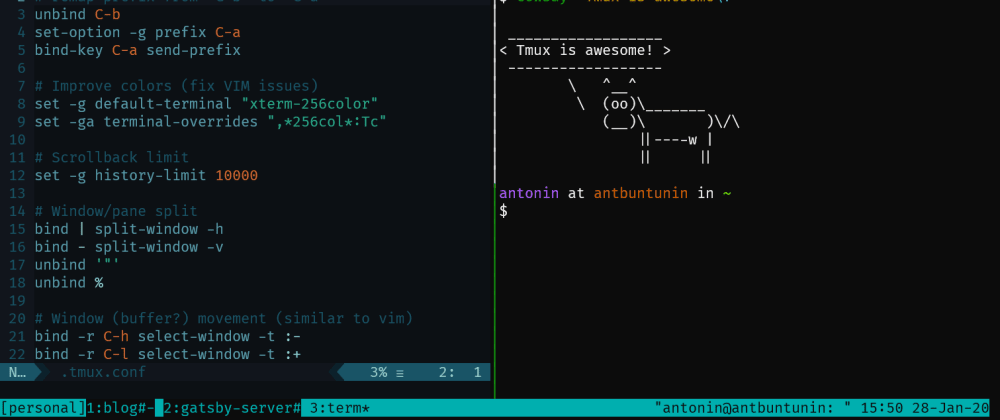
\includegraphics[scale=0.35]{tmux.png}
\end{figure}

\end{frame}

\subsection{Labels}

\begin{frame}[fragile]{Labels}
    \begin{itemize}
        \item Labels are useful to organize resources.
        \item For instance to set the Ingress for the right deployment
    \end{itemize}
    
    \begin{lstlisting}
        --labels=key1=value1
        --labels=key1=value1,key2=value2
        --labels=key1=value1[,k2=v2[,k3=v3]]
        \end{lstlisting}
    
    \begin{itemize}
        \item Resources can be easily found using the \textit{-l key=value} flag
        \item \textit{k get pods -l tier=backend}
    \end{itemize}
    
\end{frame}

\subsection{Commands}

\begin{frame}[fragile]{Commands \& Arguments}
    \begin{itemize}
        \item Just like in Docker, this declares what the container should do upon (re)starting.
        \item The CLI can put this in the spec file for you.\footnote{The comamnd should be put after the \textbf{--dry-run} and \textbf{--output} flags!}
    \end{itemize}
    
    \begin{lstlisting}
        --command -- [COMMAND] [ARGS...]
    \end{lstlisting}
    
\end{frame}

\subsection{Environmental variables \& Configmaps}

\begin{frame}[fragile]{Environmental variables (ENVs)}
    
    \begin{itemize}
    \item The CLI can also set environmental variable for you in the container
    \item Location: $spec.containers[*].env[*]$
\end{itemize}

\begin{lstlisting}
--env=key=value
\end{lstlisting}
    
\end{frame}

\begin{frame}{Challenge}
    
    \begin{itemize}
        \item Create a busybox pod and echo message ‘How are you’ and have it deleted immediately
    \end{itemize}
    
\end{frame}

\begin{frame}[fragile]{Configmaps}
    
    \begin{itemize}
    \item Configmaps contain non-confidential info in key-value pairs
    \item Pods can consume ConfigMaps as \textit{environment variables} or as \textit{configuration files in a volume}.
\end{itemize}

\begin{lstlisting}
kubectl create configmap NAME --from-literal key1=value2
\end{lstlisting}
    
\end{frame}

\begin{frame}[fragile]{Pod modification}

Use the dry-run mode
\begin{lstlisting}
  --dry-run=client -o yaml > pod.yaml
\end{lstlisting}
to send the yaml to a modifiable file!
\newline \newline
This allows us to customize the specification file.

\end{frame}

\subsection{Multi-container pods}

\begin{frame}[fragile]{Multi-container pods}
\begin{itemize}
    \item Create a specification for one pod
    \item Add the second container in the $spec.containers[*]$ array!
\end{itemize}
\end{frame}

\subsection{Configmaps}

\subsection{Security context}

\begin{frame}{Security context}
    \begin{itemize}
        \item Has to be customized manually. Look into the documentaton to prevent running pods as root!
        \begin{itemize}
            \item AllowPrivilegeEscalation=false
            \item RunAsUser=1000
            \item RunAsGroup=2000
        \end{itemize}
    \end{itemize}
\end{frame}

\section{Deployments}

\begin{frame}[fragile]{Deployment}

\begin{itemize}
    \item Deploys pods
    \item Specifies desired amount of replicas
    \item Deployment strategy
\end{itemize}

\begin{lstlisting}
kubectl create deployment NAME \ 
                          --image=image \
                          [--replicas=x] \ 
                          [options]
\end{lstlisting}

\end{frame}

\section{Services}

\begin{frame}[fragile]{Services}

Both
\begin{lstlisting}
kubectl expose [pod/deployment]
\end{lstlisting}
and 
\begin{lstlisting}
kubectl create service
\end{lstlisting}
can be used to create a service. 
\newline \newline
I prefer using kubectl expose as it is more customizable and lets kubectl check whether the service can expose the pod/deployment.

\end{frame}

\subsection{kubectl create svc}

\begin{frame}[fragile]{Services}
    
\begin{lstlisting}
$ kubectl create service --help
Create a service using a specified subcommand.

Aliases:
service, svc

Available Commands:
  clusterip    Create a ClusterIP service
  externalname Create an ExternalName service
  loadbalancer Create a LoadBalancer service
  nodeport     Create a NodePort service
\end{lstlisting}    
    
    
\end{frame}

\subsection{kubectl expose}

\begin{frame}[fragile]{Services}
    
\begin{lstlisting}
$ kubectl expose --help
Expose a resource as a new Kubernetes service.
(...)
Usage:
  kubectl expose (-f FILENAME | TYPE NAME) 
  [--port=port] [--protocol=TCP|UDP|SCTP] 
  [--target-port=number-or-name] [--name=name]
[--external-ip=external-ip-of-service] 
[--type=type] [options]
\end{lstlisting}    
    
    
\end{frame}

\end{document}
